\documentclass[a4paper]{article}
\usepackage[utf8]{inputenc}
\usepackage[T1]{fontenc}
\usepackage[pdftex]{graphicx}
\usepackage{fancyhdr}
\usepackage{lscape}
\usepackage{color}
\usepackage{qtree}
\usepackage[english]{babel}
\usepackage{graphicx}
\usepackage[colorinlistoftodos]{todonotes}
\usepackage{listings}
\usepackage{color}
\usepackage{float}
\usepackage{changepage}
\usepackage[margin=1in]{geometry}
\definecolor{codegreen}{rgb}{0,0.6,0}
\definecolor{codegray}{rgb}{0.5,0.5,0.5}
\definecolor{codepurple}{rgb}{0.58,0,0.82}
\definecolor{backcolour}{rgb}{0.95,0.95,0.92}
\usepackage[parfill]{parskip}
 \usepackage{ragged2e}
 \lstdefinestyle{mystyle}{
 	backgroundcolor=\color{backcolour},   
 	commentstyle=\color{codegreen},
 	keywordstyle=\color{magenta},
 	numberstyle=\tiny\color{codegray},
 	stringstyle=\color{codepurple},
 	basicstyle=\footnotesize,
 	breakatwhitespace=false,         
 	breaklines=true,                 
 	captionpos=b,                    
 	keepspaces=true,                 
 	numbers=left,                    
 	numbersep=5pt,                  
 	showspaces=false,                
 	showstringspaces=false,
 	showtabs=false,                  
 	tabsize=2
 }
 
\lstset{
	style=mystyle,
	inputencoding=utf8,
	extendedchars=true,
	literate={á}{{\'a}}1 {ã}{{\~a}}1 {é}{{\'e}}1,
	escapechar=\&
}
\title{Algorithmique et structures de données : Mission 3}
\date{24 octobre 2014}
\author{Groupe 1.2: Ivan Ahad - Jérôme Bertaux - Rodolphe Cambier \\ 
	Baptiste Degryse - Wojciech Grynczel - Charles Jaquet}



\begin{document}
\maketitle

\paragraph*{Question 1}
\paragraph*{Question 2 (Baptiste Degryse)}
L'algorithme de Knuth-Morris-Pratt, contrairement à l'algorithme de Boyer-Moore, a une sorte de mémoire qui va lui permettre d'identifier les caractères posant régulièrement problème, et de s'adapter afin de limiter le nombre de comparaisons. Il va éviter de refaire x fois la même erreur en comparant des lettres sans importance.\\

La complexité temporelle de cet algorithme est O(m+n), m et n étant la longueur des chaines de caractères à comparer contre une complexité temporelle O(n*m) dans l'algorithme Brute Force. Cette différence est due à la mémoire de la failure fonction dans  KMP. Cette mémoire permet de ne comparer que les caractères les plus problématiques. Exemple de l'utilisation de cette fonction:\\
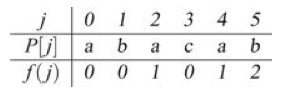
\includegraphics[scale=1]{imgFailure.png}

\paragraph*{Question 3 (Charles Jacquet)} 

Premièrement, on utilise les tries lorsque l'ont a besoin de faire une recherche d'un string dans un texte. Le problème posé est bien le même que pour la question précédente, mais la façon de faire les choses est totalement différente, c'est-à-dire que pour le KMP, on travail sur le string pattern, tandis qu'ici, on travail directement sur le texte, ce qui nous permet d'ailleurs, de faire des recherches différentes en analysant une seule fois le texte.
\begin{itemize}
\item {Compressed trie} : c'est un trie sauf que lorsqu'un noeud à un seul enfant, on rassemble le noeud et son enfant pour éviter ce qu'ils appellent les "redondances".
\item {Gain de place} : Il faut sauvegarder moins de noeud, de plus, il stock les string en dehors de l'arbre, ce qui signifie que dans l'arbre, la complexité spaciale d'un élément est en O(1).
\item {Relation entre un Trie et Suffix Tree} : Un suffix tree, est un trie pour lequel tous les strings stocké dans la collection sont suffix d'un String X.
\end{itemize}
\paragraph*{Question 4}
\paragraph*{Question 5}
\paragraph*{Question 6 (Bertaux Jérôme)}
Un algorithme de décompression d'un code de Huffman peut se décrire en deux étapes formant une fonction récursive. A chaque itération :
\begin{itemize}
\item Soit le noeud de l'arbre n'est pas une feuille donc on rappel la fonction avec le prochain bit et le fils de gauche si le bit actuel est 0 ou le fils de droite si le bit actuel est 1.
\item Soit le noeud de l'arbre est une feuille, on note alors l'élément se trouvant dans celle-ci. Et on rappel la fonction avec le bit suivant et la racine de l'arbre.
\end{itemize} 
La complexité calculatoire dépend du nombre de bits (n) et est donc de O(n). Pour effectuer l'algorithme nous avons besoin de l'arbre de priorité, d'un texte codé sur forme d'une liste de bit.

\end{document}